
\chapter{分离与固有的态射，以及（终于！）簇}
\label{ch:separated-proper}

\trSeparatedness{}是一条根本性的观念。它是\trManifold{}的\trHausdorff{}条件之类比（见\mbox{练习~11.2.B}），而且正如\trHausdorff{}性一样，这个几何上直观的观念最终恰好是让定理得以运转的那个假设。定义初看古怪，回头看却恰到好处。

我们来回顾一下为何喜欢\trHausdorff{}性。回忆：\trTopologicalSpace{}称为\trHausdorff{}的，若对任意两点 $x$ 与 $y$，都存在 $x$ 与 $y$ 的不交开邻域。实直线是\trHausdorff{}的，但「加倍原点的实直线」（图~4.6 可视为其草图）不是。关于\trManifold{}的许多证明与结果本质性地用到\trHausdorff{}性。例如，紧一维\trManifold{}的分类非常简单，但若去掉\trHausdorff{}条件，我们将面对一个非常野蛮的集合。

于是，手握这一定义，我们便可愉快地把加倍原点的直线逐出文明讨论，并且能够（终于！）按与经典定义相合的方式定义\trVariety{}的观念。

有了来自\trManifold{}的动机，我们对「一切\trAffineScheme{}与\trProjectiveScheme{}都分离」便不应感到意外。\trHausdorff{}空间的子集自动\trHausdorff。因此，若 $Y$ 是一个\trManifold，而 $X$ 是一个满足\trManifold{}除\trHausdorff{}性外全部假设的子集，则 $X$ 是\trManifold。类似地，我们将看到：\trSeparated{}对象中的\trLocally\trClosedEmbedding{}也是\trSeparated{}的（合并\mbox{练习~11.2.C}与命题~11.2.3）。

\trGrothendieck{}教导我们：应当设法把性质定义在\trMorphism{}上而非\trObject{}上；然后我们便可以说，一个\trObject{}具有该性质，如果它到\trFinalObject{}的\trMorphism{}具有该性质。我们在第~8 章开头简短地讨论过这一点。本着这一精神，\trSeparatedness{}将是\trMorphism{}的性质，而非\trScheme{}的性质。

一项意想不到的红利是：到\trAffineScheme{}的\trSeparated{}\trMorphism{}具有这样的性质——源中两个\trAffine\trOpenSet{}之交是仿射的（命题~11.2.13）。这将使 \v{C}ech 上同调在（\trQuasicompact{}）概形上运转得非常顺畅（第~18 章）。你不妨把它看作 $\mathbb{R}^n$ 中两个凸集之交仍凸这一事实的类比。由于\trAffineScheme{}从拟凝聚上同调的视角看是平凡的——恰如 $\mathbb{R}^n$ 中的凸集没有上同调——这个比喻是贴切的。

这项构造还带来一条教训：对角态射（定义~1.2.7）很重要。更确切地说，给定\trMorphism{} $\pi\colon X\to Y$，可由对角态射 $\delta_\pi\colon X\to X\times_Y X$（恒等\trMorphism{} $X\to X$ 与自身的\trFiberProduct{}）的良好行为撬出良好的结论，通常经由有趣的追图。这条教训适用于几何学的许多领域。（对角态射的另一份美好馈赠：它将在第~21 章给我们一个微分的好代数定义。）

因此，在定义\trSeparatedness{}之前，我们先对对角态射作些观察。


\section{对角态射的妙用，兼轻松搞定拟分离性}

回想：大多数\trMorphism{}类在 \S8.1 的意义下都是「合理」的：它们 (i) 对\trComposition{}保持，(ii) 对\trBaseChange{}保持\footnote{原书此处作（presesrved），当系「preserved」之误，径改。——译者注}，(iii) 对目标局部，并且作为推论，(iv) 对\trProduct{}保持（\cref{ex:property-product-preserved}）。

另一个有用的推论是：(v) 「合理」的\trMorphism{}类享有一条「\trCancellationProperty{}」（cancellation property）。这涉及那些\emph{对角态射}落在 $P$ 中的\trMorphism，也就是说，那些使得 $\delta_\pi\colon X\to X\times_Y X$ 落在 $P$ 中的\trMorphism{} $\pi\colon X\to Y$。我们把这个辅助的\trMorphism{}类称作 $P\delta$（「$P$-对角」）。

\trCancellationTheorem{}是一个看上去很怪、却极为有用的结果。正如\cref{ex:diagonal-base-change-square}的对角—基变换图一样，这个结果出人意料地无处不在。

\textbf{11.1.1.\ 关于态射性质 $P$ 的\trCancellationTheorem{}。}\ ——\ \emph{设 $P$ 是一个对\trBaseChange{}与\trComposition{}均保持的\trMorphism{}类。（每个「合理」的\trMorphism{}类都满足这一点，\S8.1。）设}
\[
\begin{tikzcd}[row sep=2.4em, column sep=3.2em]
X \ar[rr, "\pi"] \ar[dr, "\tau"'] & & Y \ar[dl, "\rho"] \\
& Z &
\end{tikzcd}
\]
\emph{是概形的一个\trCommutativeDiagram。设 $\rho$ 属于 $P\delta$，$\tau$ 属于 $P$。那么 $\pi$ 属于 $P$。}

下面的方图概括了这个重要的定理：
\[
\begin{tikzcd}[row sep=2.4em, column sep=3.2em]
X \ar[rr, "\therefore\in P"] \ar[dr, "\in P"'] & & Y \ar[dl, "\in P\delta"] \\
& Z &
\end{tikzcd}
\]

代入不同的 $P$，你就会得到面貌迥异（而且并不显然）的推论，其中第一条由\mbox{练习~11.2.E}给出。（这里有几件你很容易证明的事实，它们可以被解读为\trCancellationTheorem{}在集合的\trCategory{} $\catSets$ 中的应用，从而有助于看清\trCancellationTheorem{}为何奏效。设 $\pi\colon X\to Y$ 与 $\rho\colon Y\to Z$ 都是集合的映射。若 $\rho\circ\pi$ 是\trInjectiveMap，则 $\pi$ 亦然；若 $\rho\circ\pi$ 是\trSurjectiveMap{}而 $\rho$ 是\trInjectiveMap，则 $\pi$ 是\trSurjectiveMap。）

\textbf{11.1.A.（练习）}\quad 证明\trCancellationTheorem~11.1.1。可能的提示：解读并利用下面的方图。
\[
\begin{tikzcd}[row sep=3.4em, column sep=1.45em]
X \ar[r, equals] \ar[rrrr, bend left=17, "\therefore\in P"] &
X\times_Y Y \ar[r] \ar[dl] &
X\times_Z Y \ar[r] \ar[dl] \ar[dr] &
Z\times_Z Y \ar[r, equals] \ar[dr] &
Y \\
Y \ar[r, "\in P"] & Y\times_Z Y & & X \ar[r, "\in P"] & Z
\end{tikzcd}
\]

(vi) 若 $P$ 是一个「合理」的类，则 $P\delta$ 也是：

\textbf{11.1.2.\ \trhTheorem{}。}\ ——\ \emph{若 $P$ 是一个「合理」的\trMorphism{}类，那么由对角落在 $P$ 中的那些\trMorphism{}组成的类 $P\delta$ 也是一个「合理」的类。}

\emph{证明。}\ 我们验证：$P\delta$ 满足「合理性的三公理」。

\textbf{11.1.B.（练习）}\quad 证明：「$P\delta$ 对\trComposition{}保持」。提示：解读并利用下面的方图。
\[
\begin{tikzcd}[row sep=3em, column sep=2.9em]
X \ar[r, "\in P"] \ar[rr, bend left=28, "\therefore\in P"] &
X\times_Y X \ar[r] \ar[d] & X\times_Z X \ar[d] \\
& Y \ar[r, "\in P"] & Y\times_Z Y
\end{tikzcd}
\]

\textbf{11.1.C.（练习）}\quad 证明：「$P\delta$ 对\trBaseChange{}保持」。提示：设下面的 (a) 是\trCartesianDiagram，证明 (b) 也是\trCartesianDiagram。
\[
\text{（a）}\quad
\begin{tikzcd}[row sep=2.4em, column sep=2.9em]
\mathsf{V} \ar[r] \ar[d] & \mathsf{W} \ar[d] \\
X \ar[r] & Y
\end{tikzcd}
\qquad\qquad
\text{（b）}\quad
\begin{tikzcd}[row sep=2.4em, column sep=2.9em]
\mathsf{V} \ar[r] \ar[d] & \mathsf{V}\times_{\mathsf{W}}\mathsf{V} \ar[d] \\
X \ar[r] & X\times_Y X
\end{tikzcd}
\]

\textbf{11.1.D.（练习）}\quad 证明：「$P\delta$ 对目标局部」。提示：设我们有 $Y$ 的一个覆盖 $\{\mathsf{U}_i\to Y\}$，使得我们有一个\trCartesianDiagram{} (a)。那么我们就有\trCartesianDiagram{} (b)。
\[
\text{（a）}\quad
\begin{tikzcd}[row sep=2.4em, column sep=2.7em]
\mathsf{V}_i \ar[r, hook, "\in P\delta"] \ar[d, hook] & \mathsf{U}_i \ar[d, hook] \\
X \ar[r] & Y
\end{tikzcd}
\qquad\qquad
\text{（b）}\quad
\begin{tikzcd}[row sep=2.4em, column sep=3.1em]
\mathsf{V}_i \ar[r, "\therefore\in P"] \ar[d, hook] & \mathsf{V}_i\times_{\mathsf{U}_i}\mathsf{V}_i \ar[d] \\
X \ar[r] & X\times_Y X
\end{tikzcd}
\]
\hfill$\square$

我们继续罗列「合理」的\trMorphism{}类的有用性质。

(vii) 最后，若你有两个从 $X$ 出发、具有某种形态的\trMorphism，下一道练习将告诉你：还需要什么，才能保证到积上的那个映射也具有同样的形态。这一次，「看图证明」就留给你自己完成。

\textbf{11.1.E.（练习）}\quad 设 $P$ 是一个「合理」的\trMorphism{}类。设 $\rho\colon X\to Y$ 与 $\sigma\colon X\to Z$ 都是 $S$-\trScheme{}之间的、属于类 $P$ 的\trMorphism，而 $X\to S$ 属于 $P\delta$。证明：$(\rho,\sigma)\colon X\to Y\times_S Z$ 也属于类 $P$。（一个应用见\mbox{练习~11.2.A}。）

\textbf{11.1.F.}\ \hard\ \textbf{（练习）}\quad 证明：\trFinitelyPresented{}态射构成一个「合理」的\trMorphism{}类。

\textbf{11.1.3.\ \trhExample{}：\trMonomorphism{}。}\quad 回想：\trMorphism{} $\pi\colon X\to Y$ 是\trMonomorphism，当且仅当\trDiagonalMorphism{} $\delta_\pi\colon X\to X\times_Y X$ 是一个\trIsomorphism（\cref{ex:monomorphism-diagonal-isomorphism}）。由于\trIsomorphism{}构成一个「合理」的\trMorphism{}类，我们便立即证明了\trMonomorphism{}也构成一个「合理」类（还顺带解掉了\cref{ex:composite-of-monomorphisms}，并证明了\trMonomorphism{}对\trBaseChange{}保持）。

\textbf{11.1.4.\ 重新定义：拟分离\trMorphism{}。}

我们（现在）说：\trMorphism{} $\pi\colon X\to Y$ 是\textbf{\trQuasiSeparated}的，若\trDiagonalMorphism{} $\delta_\pi\colon X\to X\times_Y X$ 是\trQuasicompact{}的。

\textbf{11.1.G.（练习）}\quad 证明这与我们早先的拟分离定义（\S8.3.1）相一致：证明 $\pi\colon X\to Y$ 是\trQuasiSeparated{}的，当且仅当对 $Y$ 的任意\trAffine\trOpenSet{} $\Spec A$，以及 $X$ 中映入 $\Spec A$ 的两个\trAffine\trOpenSubset{} $\mathsf{U}$ 与 $\mathsf{V}$，交 $\mathsf{U}\cap\mathsf{V}$ 总是\emph{有限}多个\trAffine\trOpenSet{}之并。（可能的提示：与命题~11.2.13 相对照。另一个可能的提示：对角—基变换图，\cref{ex:diagonal-base-change-square}。）

\textbf{11.1.5.}\ 由于\trQuasicompact{}态射构成一个「合理」的类（\S10.4.E），定理~11.1.2 蕴涵：\trQuasiSeparated{}态射竟也构成一个「合理」类！特别地，\trQuasiSeparated{}态射对\trComposition{}与\trBaseChange{}保持，并且这个概念是对目标局部的。

\textbf{11.1.6.}\ 以上这番讨论出奇地置身于几何之外。为了请几何登场，我们现在更仔细地端详对角态射——它可不是随便哪一类\trMorphism。


\section{分离性与簇}

\textbf{11.2.1.\ \trhProposition{}。}\ ——\ \emph{设 $\pi\colon X\to Y$ 是概形之间的一个\trMorphism。}\\
\emph{(a) 若 $X$ 与 $Y$ 都是仿射的，那么\trDiagonalMorphism{} $\delta_\pi\colon X\to X\times_Y X$ 是一个\trClosedEmbedding。}\\
\emph{(b) 在一般情形，\trDiagonalMorphism{} $\delta_\pi\colon X\to X\times_Y X$ 是一个\trLocallyClosedEmbedding。}

$X\times_Y X$ 中与之相应的局部闭子概形——即\textbf{对角（局部闭）子概形}（diagonal (locally closed) subscheme）——将记作 $\Delta$。

\emph{证明。}\ （a）设 $X=\Spec A$，$Y=\Spec B$。于是\trDiagonalMorphism{}对应于自然的环映射 $A\otimes_B A\to A$，即由 $a_1\otimes a_2\mapsto a_1a_2$ 给出的那个映射，它显然是满射。

（b）我们将描述 $X\times_Y X$ 的一族\trOpenSubset{}，取其并来盖住 $X$ 的像，使得 $X$ 的像在这个并中是一个\trClosedEmbedding。

设 $Y$ 被\trAffine\trOpenSet{} $\mathsf{V}_i$ 所覆盖，而 $X$ 被\trAffine\trOpenSet{} $\mathsf{U}_{ij}$ 所覆盖，且 $\pi\colon\mathsf{U}_{ij}\to\mathsf{V}_i$。注意 $\mathsf{U}_{ij}\times_{\mathsf{V}_i}\mathsf{U}_{ij}$ 是积 $X\times_Y X$ 的一个\trAffine\trOpenSubscheme（我们当初构造积，基本上就是把仿射积木块粘合起来）。于是对角线被这些\trAffine\trOpenSubset{} $\mathsf{U}_{ij}\times_{\mathsf{V}_i}\mathsf{U}_{ij}$ 所覆盖。（$X$ 的任一点 $p$ 都落在某个 $\mathsf{U}_{ij}$ 中；于是 $\delta(p)\in\mathsf{U}_{ij}\times_{\mathsf{V}_i}\mathsf{U}_{ij}$。图~\ref{fig:diagonal-neighborhood} 或许有帮助。）注意 $\delta^{-1}(\mathsf{U}_{ij}\times_{\mathsf{V}_i}\mathsf{U}_{ij})=\mathsf{U}_{ij}$：一方面 $\mathsf{U}_{ij}\subset\delta^{-1}(\mathsf{U}_{ij}\times_{\mathsf{V}_i}\mathsf{U}_{ij})$ 是显然的；另一方面，由于 $\mathrm{pr}_1\circ\delta=\id_X$（其中 $\mathrm{pr}_1$ 是第一个\trProjection），又有 $\delta^{-1}(\mathsf{U}_{ij}\times_{\mathsf{V}_i}\mathsf{U}_{ij})\subset\mathsf{U}_{ij}$。最后，由 (a)，$\mathsf{U}_{ij}\to\mathsf{U}_{ij}\times_{\mathsf{V}_i}\mathsf{U}_{ij}$ 是一个\trClosedEmbedding。\hfill$\square$

\begin{figure}[htbp]
\centering
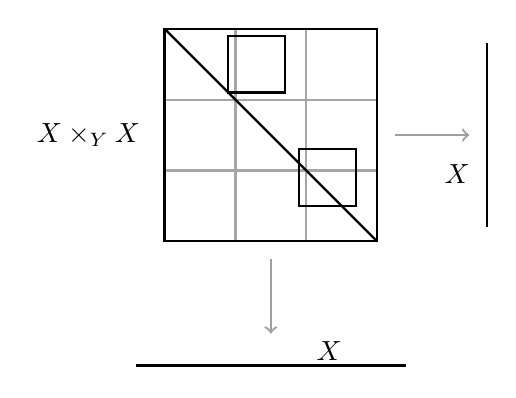
\begin{tikzpicture}[scale=0.9,line width=0.8pt]
  \draw[gray!70] (1,0) -- (1,3);
  \draw[gray!70] (2,0) -- (2,3);
  \draw[gray!70] (0,1) -- (3,1);
  \draw[gray!70] (0,2) -- (3,2);
  \draw (0,0) rectangle (3,3);
  \draw (0,3) -- (3,0);
  \draw (0.9,2.1) rectangle (1.7,2.9);
  \draw (1.9,0.5) rectangle (2.7,1.3);
  \node[anchor=east] at (-0.2,1.5) {$X\times_Y X$};
  \draw[gray!75,->] (3.25,1.5) -- (4.3,1.5);
  \draw (4.55,0.2) -- (4.55,2.8);
  \node[anchor=east] at (4.45,0.95) {$X$};
  \draw[gray!75,->] (1.5,-0.25) -- (1.5,-1.3);
  \draw (-0.4,-1.75) -- (3.4,-1.75);
  \node[anchor=west] at (2.0,-1.55) {$X$};
\end{tikzpicture}
\caption{对角线的一个开邻域被 $\mathsf{U}_{ij}\times_{\mathsf{V}_i}\mathsf{U}_{ij}$ 所覆盖。（依原书手绘图重绘。）}\label{fig:diagonal-neighborhood}
\end{figure}

我们所描述的这些开子集未必盖住 $X\times_Y X$，所以我们并没有证明 $\delta$ 是一个\trClosedEmbedding。

\textbf{11.2.A.（容易的练习）}\quad 设 $X\to Y$ 与 $X\to Z$ 都是\trLocallyClosedEmbedding。证明：$X\to Y\times Z$ 是\trLocallyClosedEmbedding。提示：\mbox{练习~11.1.E}。

\textbf{11.2.2.}\ \emph{\trhDefinition{}。}\quad \trMorphism{} $\pi\colon X\to Y$ 称为\textbf{\trSeparated}的（separated），若\trDiagonalMorphism{} $\delta_\pi\colon X\to X\times_Y X$ 是一个\trClosedEmbedding。一个 $A$-\trScheme{} $X$ 称为\textbf{在 $A$ 上\trSeparated}（separated over $A$），若\trStructureMorphism{} $X\to\Spec A$ 是\trSeparated{}的。当人们说概形（而非\trMorphism{}）$X$ 是\trSeparated{}的，他们默认指的是某个「\trStructureMorphism」是\trSeparated{}的。例如，若他们在谈论 $A$-\trScheme，他们的意思是 $X$ 在 $A$ 上\trSeparated。

多亏命题~11.2.1(b)（以及「像为闭集的\trLocallyClosedEmbedding{}实际上就是\trClosedEmbedding」这一事实，\mbox{练习~9.2.B}），\trMorphism{}是\trSeparated{}的，当且仅当对角线 $\Delta$ 是一个\trClosedSubset——这是对对角线的一条纯拓扑条件。这不禁让人想起\trHausdorff{}的一条定义，见下一道练习。

\textbf{11.2.B.（练习，仅为寻求拓扑动机的读者而设）}\quad 证明：\trTopologicalSpace{} $X$ 是\trHausdorff{}的，当且仅当对角线是 $X\times X$ 的\trClosedSubset。（概形的\trSeparatedness{}之所以不给出\trHausdorff{}性——也就是说，任意两点 $x$ 与 $y$ 未必有不相交的开\trNeighborhood——是因为在概形的\trCategory{}中，拓扑空间 $X\times X$ 一般不是拓扑空间 $X$ 与其自身的\trProduct；见 \S10.1.2。\footnote{原书此处作（for any two open points），「open」当系衍词，径删。——译者注}）

\textbf{11.2.3.\ \trhProposition{}。}\ ——\ \emph{\trSeparated{}态射构成 \S8.1 意义下的一个「合理」类——它们对\trComposition{}与\trBaseChange{}保持\footnote{原书此处作（they are by preserved），当系「they are preserved」之误，径改。——译者注}，并且这个概念是对目标局部的。}

\emph{证明。}\ \trClosedEmbedding{}这个类在这个意义下是「合理」的（\mbox{练习~10.4.A}），故由定理~11.1.2，\trSeparated{}态射亦然。\hfill$\square$

\textbf{11.2.C.（练习）}\quad 证明：\trMonomorphism{}都是\trSeparated{}的。从而\trLocallyClosedEmbedding（特别地，\trOpenEmbedding{}与\trClosedEmbedding）都是\trSeparated{}的。

\textbf{11.2.D.（练习）}\quad 证明：\trSeparated{}态射都是\trQuasiSeparated{}的。（提示：\trClosedEmbedding{}都是仿射的，从而是\trQuasicompact{}的。）

\textbf{11.2.4.\ \trhProposition{}。}\ ——\ \emph{仿射态射都是\trSeparated{}的。特别地，有限态射都是\trSeparated{}的。}

\emph{证明。}\ 由命题~11.2.1(a)，仿射概形之间的每个\trMorphism{}都是\trSeparated{}的。\trSeparatedness{}这个概念是对目标局部的，故得证。\hfill$\square$

下面的许多道练习都会让你切身体会到\trCancellationTheorem~11.1.1 的重要性。

\textbf{11.2.E.（练习）}\quad 证明：一个 $A$-\trScheme{}是\trSeparated{}的（在 $A$ 上），当且仅当它在 $\mathbb{Z}$ 上\trSeparated。特别地，一个复概形在 $\mathbb{C}$ 上\trSeparated，当且仅当它在 $\mathbb{Z}$ 上\trSeparated，所以复几何学家与算术几何学家可以毫无混淆地互谈\trSeparated{}概形。

\textbf{11.2.F.（容易的练习）}\quad 设有态射 $X\xrightarrow{\ \pi\ }Y\xrightarrow{\ \rho\ }Z$。\\
(a) 证明：若 $\rho\circ\pi$ 是\trLocallyClosedEmbedding（相应地，\trLocally\trFiniteType、\trSeparated），则 $\pi$ 亦然。\\
(b) 若 $\rho\circ\pi$ 是\trQuasicompact{}的，而 $Y$ 是\trNoetherian{}的，证明 $\pi$ 是\trQuasicompact{}的。提示：\cref{ex:quasicompact-quasiseparated-source}(a)。\\
(c) 若 $\rho\circ\pi$ 是\trQuasiSeparated{}的，证明 $\pi$ 是\trQuasiSeparated{}的。提示：\cref{ex:quasicompact-quasiseparated-source}(b)。

\textbf{11.2.G.（练习）}\quad 设 $\mu\colon Z\to X$ 是一个\trMorphism，而 $\sigma\colon X\to Z$ 是 $\mu$ 的一个\trSection，即 $\mu\circ\sigma$ 是 $X$ 上的恒等。
\[
\begin{tikzcd}[row sep=3.2em]
Z \ar[dd, "\mu", bend right=16] \\
& \\
X \ar[uu, "\sigma"', bend right=16]
\end{tikzcd}
\]
证明：$\sigma$ 是一个\trLocallyClosedEmbedding。证明：若 $\mu$ 是\trSeparated{}的，则 $\sigma$ 是一个\trClosedEmbedding。证明：若 $\mu$ 是\trQuasiSeparated{}的，则 $\sigma$ 是\trQuasicompact{}的。举出一个例子，说明当 $\mu$ 不\trSeparated{}时，$\sigma$ 未必是\trClosedEmbedding。

\textbf{11.2.5.}\ \emph{\trGraphMorphism{}。}\quad 设 $\pi\colon X\to Y$ 是 $Z$-\trScheme{}之间的一个\trMorphism。由 $\gamma_\pi=(\id,\pi)$ 给出的\trMorphism{} $\gamma_\pi\colon X\to X\times_Z Y$ 称为\textbf{\trGraphMorphism{}}（graph morphism）（见图~\ref{fig:graph-morphism}）。（它曾秘密地出现在\mbox{练习~11.1.A}中。）于是 $\pi$ 可分解为 $\mathrm{pr}_2\circ\gamma_\pi$，其中 $\mathrm{pr}_2$ 是第二个\trProjection。图~\ref{fig:graph-morphism} 中的方图常被称为\textbf{态射 $\pi$ 的图像}（graph）。（我们将在 \S11.3.4 中讨论有理映射的图像。）把\mbox{练习~11.2.G}应用到 $X\times_Z Y\to X$ 上，便得到：

\begin{figure}[htbp]
\centering
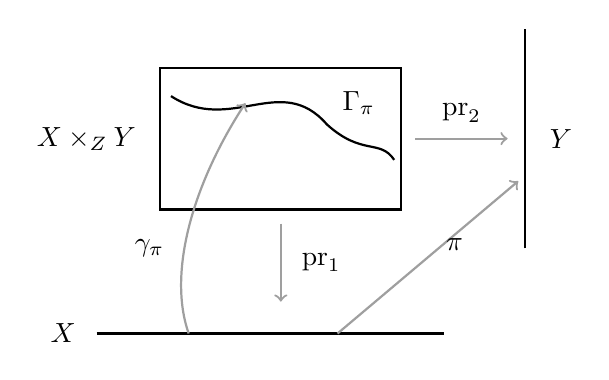
\begin{tikzpicture}[scale=0.9,line width=0.8pt]
  \draw (0,0) rectangle (3.4,2.0);
  \draw (0.15,1.6) .. controls (1.0,1.05) and (1.7,1.95) .. (2.35,1.2)
        .. controls (2.85,0.75) and (3.1,1.0) .. (3.3,0.7);
  \node at (2.8,1.5) {$\Gamma_\pi$};
  \node[anchor=east] at (-0.2,1.0) {$X\times_Z Y$};
  \draw[gray!75,->] (3.6,1.0) -- (4.9,1.0);
  \node[anchor=south] at (4.25,1.08) {$\mathrm{pr}_2$};
  \draw (5.15,-0.55) -- (5.15,2.55);
  \node[anchor=west] at (5.35,1.0) {$Y$};
  \draw[gray!75,->] (1.7,-0.2) -- (1.7,-1.3);
  \node[anchor=west] at (1.85,-0.75) {$\mathrm{pr}_1$};
  \draw (-0.9,-1.75) -- (4.0,-1.75);
  \node[anchor=east] at (-1.05,-1.75) {$X$};
  \draw[gray!75,->] (0.4,-1.75) .. controls (0.1,-0.9) and (0.45,0.35) .. (1.2,1.5);
  \node[anchor=east] at (0.2,-0.55) {$\gamma_\pi$};
  \draw[gray!75,->] (2.5,-1.75) -- (5.05,0.4);
  \node at (4.15,-0.5) {$\pi$};
\end{tikzpicture}
\caption{\trGraphMorphism{}。（依原书手绘图重绘。）}\label{fig:graph-morphism}
\end{figure}

\textbf{11.2.6.\ \trhProposition{}。}\ ——\ \emph{\trGraphMorphism{} $\gamma_\pi$ 总是一个\trLocallyClosedEmbedding。若 $Y$ 是\trSeparated{}的 $Z$-\trScheme（即 $Y\to Z$ 是\trSeparated{}的），则 $\gamma_\pi$ 是一个\trClosedEmbedding。若 $Y$ 是\trQuasiSeparated{}的 $Z$-\trScheme，则 $\gamma_\pi$ 是\trQuasicompact{}的。}

$\gamma_\pi$ 的像（$X\times_Z Y$ 的一个局部闭子概形）也常被称为 $\pi$ 的\textbf{图像}（graph of $\pi$）；我们可以把它记作 $\Gamma_\pi$。

\textbf{11.2.H.（我们不会用到的练习）}\quad 设 $P$ 是一个\trMorphism{}类：\trClosedEmbedding{}都在 $P$ 中，且 $P$ 对\trFiberProduct{}与\trComposition{}保持。回想关于态射「\trReduction」的定义~10.7.8。证明：若 $\pi\colon X\to Y$ 属于 $P$，则 $\pi^{\mathrm{red}}\colon X^{\mathrm{red}}\to Y^{\mathrm{red}}$ 属于 $P$。（两个例子是\trSeparated{}态射类与\trQuasiSeparated{}态射类。）可能的提示：
\[
\begin{tikzcd}[row sep=2.6em, column sep=3.4em]
X^{\mathrm{red}} \ar[r, "\pi^{\mathrm{red}}"] \ar[d, "\in P"'] \ar[dr] &
Y^{\mathrm{red}} \ar[d, "\in P\delta"] \\
X \ar[r, "\pi\in P"'] & Y.
\end{tikzcd}
\]

\textbf{11.2.7.\ 重要的例子。}

\textbf{11.2.I.（练习）}\quad 证明：原点加倍了的\trAffineLine（例~4.4.5）不是\trSeparated{}的，办法是验证\trDiagonalMorphism{}的像不是\trClosedSubset。（下文的\mbox{练习~11.3.C}给出另一个论证；\mbox{练习~13.7.C}将给出一个花哨的论证。）

我们马上迎来第一个「\trSeparated{}但不仿射」的例子。下面这区区一步计算就将蕴涵：所有拟射影 $A$-\trScheme{}都是\trSeparated{}的（一旦我们知道\trSeparated{}态射的\trComposition{}仍是\trSeparated{}的，命题~11.2.3）。

\textbf{11.2.8.\ \trhProposition{}。}\ ——\ \emph{态射 $\mathbb{P}^n_A\to\Spec A$ 是\trSeparated{}的。}

我们给出两个证明。第一个靠直接计算；第二个无须任何计算，只要求你记得前面讲过的一些经典构造。

\emph{证明~1：直接计算。}\ 我们用形如 $\mathsf{U}_i\times_A\mathsf{U}_j$ 的开集覆盖 $\mathbb{P}^n_A\times_A\mathbb{P}^n_A$，其中 $\mathsf{U}_0,\dots,\mathsf{U}_n$ 构成「通常的」\trAffine\trOpenCover。$i=j$ 的情形此前已在命题~11.2.1(a) 的证明中处理过。若 $i\neq j$，则
\[
\mathsf{U}_i\times_A\mathsf{U}_j\cong\Spec A[x_{0/i},\dots,x_{n/i},\,y_{0/j},\dots,y_{n/j}]/(x_{i/i}-1,\ y_{j/j}-1).
\]
现在 $\delta^{-1}(\mathrm{pr}_1^{-1}(\mathsf{U}_i))$ 就是 $\mathsf{U}_i$（因为\trDiagonalMorphism{}与到第一个因子的\trProjection{}复合是恒等映射），类似地 $\mathsf{U}_j=\delta^{-1}(\mathrm{pr}_2^{-1}(\mathsf{U}_j))$。于是 $\delta^{-1}(\mathsf{U}_i\times_A\mathsf{U}_j)=\mathsf{U}_i\cap\mathsf{U}_j$，所以在 $\mathsf{U}_i\times_A\mathsf{U}_j$ 上的\trDiagonalMorphism{}就是 $\mathsf{U}_i\cap\mathsf{U}_j\to\mathsf{U}_i\times_A\mathsf{U}_j$。这是一个\trClosedEmbedding，因为相应的环映射
\[
A[x_{0/i},\dots,x_{n/i},y_{0/j},\dots,y_{n/j}]
\longrightarrow
A[x_{0/i},\dots,x_{n/i},x_{j/i}^{-1}]/(x_{i/i}-1)
\]
（由 $x_{k/i}\mapsto x_{k/i}$、$y_{k/j}\mapsto x_{k/i}/x_{j/i}$ 给出）显然是满射（右边的环的每个生成元都显然落在像中——注意 $x_{j/i}^{-1}$ 是 $y_{i/j}$ 的像）。\hfill$\square$

\emph{证明~2：经典几何。}\ 注意：\trDiagonalMorphism{} $\delta\colon\mathbb{P}^n_A\to\mathbb{P}^n_A\times_A\mathbb{P}^n_A$ 复合上 \trSegre{}嵌入 $S\colon\mathbb{P}^n_A\times_A\mathbb{P}^n_A\to\mathbb{P}^{n^2+2n}$（\S10.6，一个\trClosedEmbedding）之后，也可以分解为第二个\trVeroneseEmbedding{} $v_2\colon\mathbb{P}^n_A\to\mathbb{P}^{\binom{n+2}{2}-1}$（\S9.3.6）与一个线性映射 $L\colon\mathbb{P}^{\binom{n+2}{2}-1}\to\mathbb{P}^{n^2+2n}$ 的复合，而这两者都是\trClosedEmbedding（线性映射 $L$ 的情形由\mbox{练习~9.3.C}给出）。
\[
\begin{tikzcd}[row sep=2.9em, column sep=3.4em]
& \mathbb{P}^n_A\times_A\mathbb{P}^n_A
  \ar[dl, "\delta", "\text{局部（？）闭嵌入}"'] \ar[dr, "S", "\text{闭嵌入}"'] & \\
\mathbb{P}^n_A \ar[dr, "v_2"', "\text{闭嵌入}"'] & & \mathbb{P}^{n^2+2n} \\
& \mathbb{P}^{\binom{n+2}{2}-1} \ar[ur, "L"', "\text{闭嵌入}"'] &
\end{tikzcd}
\]
不严格地说，用坐标来看：
{\small
\[
\begin{tikzcd}[row sep=3.2em, column sep=2.2em]
& \bigl([x_0,x_1,\dots,x_n],\,[x_0,x_1,\dots,x_n]\bigr)
  \ar[dl, "\delta"'] \ar[dr, "S"] & \\
{[x_0,x_1,\dots,x_n]} \ar[dr, "v_2"'] & &
{\begin{bmatrix}
x_0^2 & x_0x_1 & \cdots & x_0x_n \\
x_1x_0 & x_1^2 & \cdots & x_1x_n \\
\vdots & \vdots & \ddots & \vdots \\
x_nx_0 & x_nx_1 & \cdots & x_n^2
\end{bmatrix}} \\
& {[x_0^2,x_0x_1,\dots,x_{n-1}x_n,x_n^2].} \ar[ur, "L"'] &
\end{tikzcd}
\]
}
复合映射 $\mathbb{P}^n_A\to\mathbb{P}^{n^2+2n}$ 可以写成
\[
[x_0,\dots,x_n]\mapsto[x_0^2,\,x_0x_1,\,x_0x_2,\,\dots,\,x_n^2],
\]
其中右边的下标跑遍一切满足 $0\le i,j\le n$ 的有序对 $(i,j)$。这就迫使 $\delta$ 把闭集送到闭集（否则 $S\circ\delta$ 就不会如此，而 $L\circ v_2$ 会）。\hfill$\square$

\textbf{11.2.9.\ 重要的定义（终于！）。}\quad 域 $k$ 上的一个\textbf{\trVariety}（variety），或称 \textbf{$k$-\trVariety}（$k$-variety），是 $k$ 上一个既约、\trSeparated{}的有限型概形。例如，既约的有限型仿射 $k$-\trScheme{}就是一个\trVariety。（你看出\trSeparatedness{}为何成立了吗？）\trVariety{}这个观念推广了我们早先的仿射簇（\S5.3.7）与射影簇（\S5.3.7；见推论~11.2.15）的观念。由\mbox{练习~5.3.F}，\trVariety{}的\trClosedPoint{}是\trDense{}的。（记号警示：在另一些文献里，还会附加\trIrreducibility{}这条条件；此外也常假定 $k$ 是\trAlgClosedField。）

$k$ 上的\trVariety{}构成一个\trCategory{}：$k$-\trVariety{}之间的\trMorphism{}就是作为 $k$-\trScheme{}的\trMorphism{}。（当然，代数闭域 $k$ 上的\trVariety{}的\trCategory{}，远在现代\trSchemeTheory{}之前就早已存在。）

\textbf{11.2.J.（容易的练习）}\quad 证明：$k$-\trVariety{}之间的\trMorphism{}都是有限型的，并且是\trSeparated{}的。

\trVariety{} $X$ 的一个\textbf{\trSubvariety{}}（subvariety）是 $X$ 的一个\emph{既约}局部闭子概形（你可以很快验证：它本身就是\trVariety）。$X$ 的开\trSubvariety{}是 $X$ 的一个\trOpenSubscheme（此时既约性是自动的）。$X$ 的闭\trSubvariety{}是 $X$ 的一个既约\trClosedSubscheme。

\textbf{11.2.K.}\ \extrahard\ \textbf{（练习，面向背景合适的读者：复代数簇给出复解析簇）}\quad 证明：复代数簇的\trAnalytification{}（\mbox{练习~7.3.P}）是一个复解析簇。

\textbf{11.2.10.\ \trVariety{}的\trProduct{}。}

\textbf{11.2.11.\ \trhProposition{}。}\ ——\ \emph{(a) 若 $k$ 是\trPerfectField，则 $k$-\trVariety{}的\trProduct（$\Spec k$ 上的\trFiberProduct）是一个 $k$-\trVariety。}\\
\emph{(b) 若 $k$ 是\trAlgClosedField，则不可约 $k$-\trVariety{}的\trProduct{}是一个不可约 $k$-\trVariety。}\\
\emph{(c) 若 $k$ 是\trAlgClosedField，则连通 $k$-\trVariety{}的\trProduct{}是一个连通 $k$-\trVariety。}

\emph{证明。}\ (a) 有限型与\trSeparated{}这两条陈述是直截了当的，因为这两条性质都对\trBaseChange{}与\trComposition{}保持。至于既约性：先化归到仿射情形，再用推论~10.5.23。

(b) 只剩下证明不可约性。用\mbox{练习~10.5.N}化归到仿射情形（如命题~10.5.15 的证明那样），再用\mbox{练习~10.5.M}，后者需要可分闭包。（作为练习，你可以改用\mbox{练习~10.4.H}，从而避开 \S10.5 的种种繁难。）

\textbf{11.2.L.（练习）}\quad 证明 (c)。\hfill$\square$

\textbf{11.2.12.\ 回到\trSeparatedness{}。}\quad 这里是\trSeparatedness{}的一条非常顺手的推论。

\textbf{11.2.13.\ \trhProposition{}。}\ ——\ \emph{设 $X\to\Spec A$ 是向一个\trAffineScheme{}的\trSeparated{}态射，而 $\mathsf{U}$ 与 $\mathsf{V}$ 是 $X$ 的\trAffine\trOpenSubset。那么 $\mathsf{U}\cap\mathsf{V}$ 是 $X$ 的一个仿射开子集。}

在证明之前，先给出一条出人意料的推论。取 $X=\Spec A$，我们便看到：$\Spec A$ 的任意两个仿射开子集的交也是仿射开子集。这一点当然绝不显然！我们知道两个特异仿射开子集的交是仿射的（由 $D(f)\cap D(g)=D(fg)$），但对一般的仿射开子集，我们几乎束手无策。

\trhWarning{}：这条性质并不刻画\trSeparatedness{}。（正确的性质是「\trAffineDiagonal{}」（affine-diagonal），我们将不讨论它，但它在\trStack{}理论中很有用。）例如，若 $A$ 是域 $k$，而 $X$ 是 $k$ 上原点加倍了的\trAffineLine，则 $X$ 也具有这条性质。

在命题~11.2.13 的证明中，我们将用到下面这个漂亮的结果。

\textbf{11.2.M.（容易的练习）}\quad 设 $\mathsf{U}$ 与 $\mathsf{V}$ 是 $A$-\trScheme{} $X$ 的\trOpenSubset。证明：$\mathsf{U}\cap(\mathsf{U}\times_A\mathsf{V})\cong\mathsf{U}\cap\mathsf{V}$。（两个局部闭子概形的交，其定义见\cref{ex:intersection-locally-closed-embeddings}。）提示：(i) 这在命题~11.2.8 的证明~1 的过程中已被基本证明。(ii) 见图~\ref{fig:diagonal-intersection}。(iii) 你可以用对角—基变换图（\cref{ex:diagonal-base-change-square}）来解读这条陈述：
\[
\begin{tikzcd}[row sep=2.4em, column sep=3.2em]
\mathsf{U}\cap\mathsf{V} \ar[r] \ar[d] & \mathsf{U}\times_A\mathsf{V} \ar[d] \\
X \ar[r, "\delta"'] & X\times_A X.
\end{tikzcd}
\]

\begin{figure}[htbp]
\centering
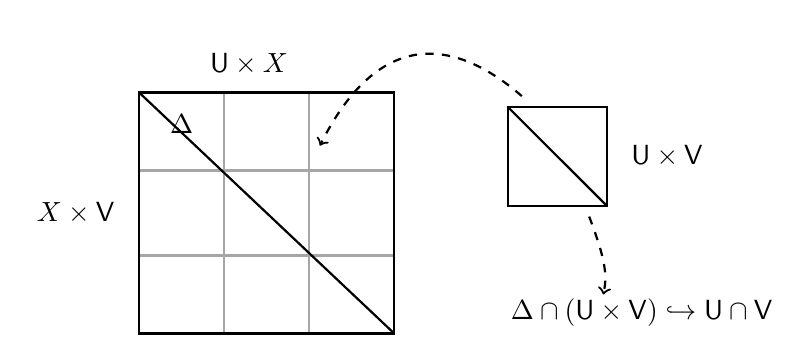
\begin{tikzpicture}[scale=0.9,line width=0.8pt]
  \draw[gray!70] (1.2,0) -- (1.2,3.4);
  \draw[gray!70] (2.4,0) -- (2.4,3.4);
  \draw[gray!70] (0,1.1) -- (3.6,1.1);
  \draw[gray!70] (0,2.3) -- (3.6,2.3);
  \draw (0,0) rectangle (3.6,3.4);
  \draw (0,3.4) -- (3.6,0);
  \node at (0.6,2.95) {$\Delta$};
  \node[anchor=south] at (1.55,3.5) {$\mathsf{U}\times X$};
  \node[anchor=east] at (-0.2,1.7) {$X\times\mathsf{V}$};
  \draw (5.2,1.8) rectangle (6.6,3.2);
  \draw (5.2,3.2) -- (6.6,1.8);
  \node[anchor=west] at (6.8,2.5) {$\mathsf{U}\times\mathsf{V}$};
  \draw[dashed,->] (5.4,3.35) .. controls (4.3,4.3) and (3.3,4.15) .. (2.55,2.65);
  \draw[dashed,->] (6.35,1.65) .. controls (6.6,1.0) and (6.6,0.8) .. (6.55,0.55);
  \node[anchor=west] at (5.1,0.3) {$\Delta\cap(\mathsf{U}\times\mathsf{V})\hookrightarrow\mathsf{U}\cap\mathsf{V}$};
\end{tikzpicture}
\caption{$\Delta\cap(\mathsf{U}\times\mathsf{V})\cong\mathsf{U}\cap\mathsf{V}$（\mbox{练习~11.2.M}）。（依原书手绘图重绘。）}\label{fig:diagonal-intersection}
\end{figure}

\textbf{11.2.14.}\ \emph{命题~11.2.13 的证明。}\quad 由\mbox{练习~11.2.M}，$(\mathsf{U}\times_A\mathsf{V})\cap\Delta\cong\mathsf{U}\cap\mathsf{V}$，其中 $\Delta$ 是对角线。但 $\mathsf{U}\times_A\mathsf{V}$ 是仿射的（两个仿射概形在仿射概形上的\trFiberProduct{}是仿射的：见我们构造纤维积的第 1 步，定理~10.1.1），而 $(\mathsf{U}\times_A\mathsf{V})\cap\Delta$ 是仿射概形 $\mathsf{U}\times_A\mathsf{V}$ 的一个\trClosedSubscheme，从而 $\mathsf{U}\cap\mathsf{V}$ 是仿射的。\hfill$\square$

\textbf{11.2.15.\ \trhCorollary{}。}\ ——\ \emph{每个拟射影 $A$-\trScheme{}都在 $A$ 上\trSeparated。特别地，每个既约的拟射影 $k$-\trScheme{}都是一个 $k$-\trVariety。}

\emph{证明。}\ 设 $X\to\Spec A$ 是一个拟射影 $A$-\trScheme。\trStructureMorphism{}可以分解为一个\trOpenEmbedding{}复合一个\trClosedEmbedding{}再复合 $\mathbb{P}^n_A\to\Spec A$。\trOpenEmbedding{}与\trClosedEmbedding{}都是\trSeparated{}的（\mbox{练习~11.2.C}），而 $\mathbb{P}^n_A\to\Spec A$ 是\trSeparated{}的（命题~11.2.8）。\trSeparated{}态射的\trComposition{}仍是\trSeparated{}的（命题~11.2.3），故得证。\hfill$\square$

下面是一道我们用不上、但你或许会喜欢的练习。它包含命题~11.2.13 的一个逆命题。

\textbf{11.2.N.（练习）}\quad 证明：$X\to\Spec A$ 是\trSeparated{}的，当且仅当对 $X$ 的所有\trAffine\trOpenSubset{} $\mathsf{U}$ 与 $\mathsf{V}$：(i) 交 $\mathsf{U}\cap\mathsf{V}$ 是仿射的，(ii) 映射 $\OO(\mathsf{U})\otimes_A\OO(\mathsf{V})\to\OO(\mathsf{U}\cap\mathsf{V})$ 是满射。证明：当 $\mathsf{U}$ 与 $\mathsf{V}$ 取遍任一\trAffine\trCover{} $X=\bigcup\mathsf{U}_i$ 中的集合时，检验上述两点就够了。（提示：命题~11.2.8 的证明~1 已把这件事做了大半。）

\textbf{11.2.16.}\ \extrahard\ \textbf{泛单射\trMorphism{}与对角线。}

\textbf{11.2.O.（练习）}\quad 证明：$\pi\colon X\to Y$ 是\textbf{\trUniversallyInjective}的（universally injective），当且仅当\trDiagonalMorphism{} $\delta_\pi\colon X\to X\times_Y X$ 是满态射。（回想：由命题~11.2.1(b)，$\delta_\pi$ \emph{总是}单的。）

由于满态射构成一个「合理」类（\mbox{练习~10.4.G}），我们看到泛单射态射也构成一个「合理」类。

\textbf{11.2.P.（容易的练习）}\quad 若 $\pi\colon X\to Y$ 与 $\rho\colon Y\to Z$ 是\trMorphism，而 $\rho\circ\pi$ 是泛单射的，证明 $\pi$ 是泛单射的。

\textbf{11.2.Q.（练习）}\\
(a) 证明：泛单射态射都是\trSeparated{}的。\\
(b) 证明：\trAlgClosedField{} $\overline{k}$ 上两个有限型概形之间的映射是泛单射的，当且仅当它在\trClosedPoint{}上是\trInjectiveMap。


\section{两个态射相等之处，与「既约到分离」定理}

我们在 \S7.5 引入\trRationalMap{}时曾经许诺：在良好的情形下，一个\trRationalMap{}拥有一个「最大的\trDomainOfDefinition」。现在，我们终于可以把「良好的情形」说精确了，办法正是「既约到分离」定理~11.3.2。我们首先引入一个重要的结果，让「源与目标皆相同的两个\trMorphism{}『相等』之处」这一说法有了确切含义。

\textbf{11.3.A.（有用的练习：两个态射相等之处）}\quad 设 $\pi\colon X\to Y$ 与 $\pi'\colon X\to Y$ 是某个概形 $Z$ 上的两个\trMorphism。
\[
\begin{tikzcd}[row sep=2.2em]
X \ar[rr, bend left=17, "\pi"] \ar[rr, bend right=17, "\pi'"'] \ar[dr] & & Y \ar[dl] \\
& Z &
\end{tikzcd}
\]
现在我们可以给「$\pi$ 与 $\pi'$ 相等之处」这一说法以确切含义了；特别地，还可以谈这样一个事实：存在一个最大的局部闭子概形使二者在其上相等——而当 $Y$ 在 $Z$ 上\trSeparated{}时，它还是闭的。设 $\mu\colon W\to X$ 是某个\trMorphism（不必假设它是局部闭嵌入）。若 $\pi\circ\mu=\pi'\circ\mu$，就说 $\pi$ 与 $\pi'$ 在 $\mu$ 上相等。证明：存在一个局部闭子概形 $\iota\colon\mathsf{V}\hookrightarrow X$，使 $\pi$ 与 $\pi'$ 在其上相等，并且任何使 $\pi$ 与 $\pi'$ 在其上相等的\trMorphism{} $\mu\colon W\to X$ 都唯一地穿过 $\iota$ 分解，也就是说，存在唯一的 $j\colon W\to\mathsf{V}$ 使 $\mu=\iota\circ j$。再证明：若 $Y\to Z$ 是\trSeparated{}的，则 $\iota\colon\mathsf{V}\hookrightarrow X$ 是一个\trClosedEmbedding。

提示：把 $\mathsf{V}$ 定义为如下的\trFiberProduct{}：
\[
\begin{tikzcd}[row sep=2.6em, column sep=3.4em]
\mathsf{V} \ar[r] \ar[d] & Y \ar[d, "\delta"] \\
X \ar[r, "{(\pi,\pi')}"'] & Y\times_Z Y.
\end{tikzcd}
\]
由于 $\delta$ 是\trLocallyClosedEmbedding，$\mathsf{V}\to X$ 亦然。于是，若 $\mu\colon W\to X$ 是任一满足 $\pi\circ\mu=\pi'\circ\mu$ 的\trMorphism，则 $\mu$ 穿过 $\mathsf{V}$。

两个映射相等之处可以不\trReduced{}，这不该令人吃惊：考虑从 $\mathbb{A}^1_k$ 到其自身的两个映射 $\pi(x)=0$ 与 $\pi'(x)=x^2$。它们在 $x=0$ 处相等，但情形（按 $\epsilon$ 的标准来衡量）还要更好——它们甚至应当在 $\Spec k[x]/(x^2)$ 上相等。\footnote{译注：epsilonically 系作者生造的词，把幂零增厚戏称为「$\epsilon$ 层次」的分辨本领：能分辨到 $\Spec k[x]/(x^2)$，就比只分辨底层点又精确了一步。}

\textbf{11.3.1.}\ \emph{小注记。}\quad (i) 在上一道练习中，我们用\trUniversalProperty{}描述了 $\mathsf{V}\to X$。若径以之为定义，那么 $\mathsf{V}$ 是 $X$ 的局部闭子概形——甚至它存在与否——都不是先验显然的。

(ii) \trhWarning{}：考虑 $\Spec\mathbb{C}$ 到自身、在 $\Spec\mathbb{R}$ 之上的两个映射：恒同与\trComplex\trConjugate。二者都是从点到点的映射，然而尽管作为集合的映射相等，它们却不相等。（若你不信它们作为\trMorphism{}并不相等，下面这话或许有帮助：经过\trBaseChange{} $\Spec\mathbb{C}\to\Spec\mathbb{R}$ 之后，它们连作为集合的映射都不相等了。）

(iii) 更一般地，$\pi$ 与 $\pi'$ 相等的（集合论）轨迹可以这样解读：$\pi$ 与 $\pi'$ 在点 $p$ 处相等，是指 $\pi(p)=\pi'(p)$，且由此给出的两个\trResidueField{}之间的映射相同。（你也许会乐于把这件事当作一道练习想个明白。\footnote{原书此处作（You may enjoying thinking），当系「enjoy」之误，径改。——译者注}）

\textbf{11.3.B.（练习：$\overline{K}$-\trVariety{}由闭点上的映射决定）}\quad 设 $\pi\colon X\to Y$ 与 $\pi'\colon X\to Y$ 是两个 $\overline{K}$-\trVariety{}之间的\trMorphism，它们在闭点的层面上相同（也就是说，对每个\trClosedPoint{} $p\in X$ 都有 $\pi(p)=\pi'(p)$）。证明：$\pi=\pi'$。（这蕴含：从「$\overline{K}$ 上的经典簇」这一\trCategory——我们不在此定义它——到 $\overline{K}$-\trScheme{}的\trCategory{}的\trFunctor{}是\trFullyFaithful{}的。你能把它恰当地推广到非\trAlgClosedField{}的情形吗？）

\textbf{11.3.C.（较不重要的练习）}\quad 证明：原点加倍了的\trAffineLine{} $X$（例~4.4.5）不是\trSeparated{}的，办法是找出两个\trMorphism{} $\pi\colon W\to X$、$\pi'\colon W\to X$，使得二者的「相等定义域」不是\trClosedSubscheme（对比\mbox{命题~11.2.1(b)}）。（\mbox{练习~11.2.I}已在上文给出另一个论证；\mbox{练习~13.7.C}将给出一个花哨的论证。）

现在我们来到本节的中心结果。

\textbf{11.3.2.\ 「既约到分离」定理}（Reduced-to-Separated Theorem）\textbf{。}\ ——\ \emph{从一个\trReduced\trScheme{}到一个\trSeparated{}的 $S$-\trScheme{}的两个 $S$-态射 $\pi\colon\mathsf{U}\to Z$、$\pi'\colon\mathsf{U}\to Z$，若在 $\mathsf{U}$ 的一个\trDense\trOpenSubset{}上相等，则二者相同。}

\emph{证明。}\ 令 $\mathsf{V}$ 为 $\pi$ 与 $\pi'$ 相等之处。它是 $\mathsf{U}$ 的一个\trClosedSubscheme（由\mbox{练习~11.3.A}），并且含有一个稠密开集。但既约概形 $\mathsf{U}$ 的\trClosedSubscheme{}之中，底集合稠密者唯有 $\mathsf{U}$ 自身。（你看出最后这句话为什么成立吗？若去掉既约性假设，你能给出反例吗？）\hfill$\square$

\textbf{11.3.3.}\quad \emph{推论~1。}\ 于是（由于 $X$ 既约、$Y$ 分离），若有两个从 $X$ 的开子集出发、到 $Y$ 的\trMorphism，比如说 $\pi\colon\mathsf{U}\to Y$ 与 $\pi'\colon\mathsf{V}\to Y$，并且它们在 $\mathsf{U}\cap\mathsf{V}$ 的一个稠密开子集 $Z$ 上相等，那么它们必在 $\mathsf{U}\cap\mathsf{V}$ 上相等。

\emph{推论~2。}\ 一个\trRationalMap{}拥有一个最大的\trDomainOfDefinition{}——$\pi\colon\mathsf{U}\dashrightarrow Y$ 在其上是一个\trMorphism{}——它就是全部\trDomainOfDefinition{}之并。特别地，\trReduced\trScheme{}上的\trRationalFunction{}拥有一个最大的\trDomainOfDefinition。例如，由 $(x,y)\mapsto[x,y]$ 给出的\trRationalMap{} $\mathbb{A}^2_k\dashrightarrow\mathbb{P}^1_k$，其\trDomainOfDefinition{}为 $\mathbb{A}^2_k\setminus\{(0,0)\}$（参看 \S7.5.3）。这在部分程度上推广了\trLocally\trNoetherian{}概形上\trRationalFunction{}之定义域的观念（定义~6.6.36）。\trDomainOfDefinition{}的补集称为\textbf{\trIndeterminacyLocus}（indeterminacy locus；这一说法早先已在 \S6.6.36 中使用过），它的点有时被称为该\trRationalMap{}的\textbf{\trFundamentalPoint{}}（fundamental points），不过我们不会使用这些说法。（我们将在\mbox{练习~22.4.L}中看到：到\trProjectiveScheme{}的\trRationalMap{}可以通过「胀开」一个概形论版本的不定性轨迹，升级为一个名副其实的\trMorphism。）

\textbf{11.3.D.（练习）}\quad 证明：若放弃源的既约性或目标的分离性，「既约到分离」定理~11.3.2 便不成立。这里给出几种可能。对于第一种，考虑从 $\Spec k[x,y]/(y^2,xy)$ 到 $\Spec k[t]$ 的两个映射，其中 $\pi$ 由 $t\mapsto x$ 给出，$\pi'$ 由 $t\mapsto x+y$ 给出；$\pi$ 与 $\pi'$ 在由 $y=0$ 切出的\trClosedSubscheme{}上相等。对于第二种，考虑从 $\Spec k[t]$ 到原点加倍了的\trAffineLine{}的两个映射，其一映入「上半」，另一映入「下半」。这两个\trMorphism{}在稠密开集 $D(t)$ 上相等；见图~\ref{fig:nonseparated-agreement}。

\begin{figure}[htbp]
\centering
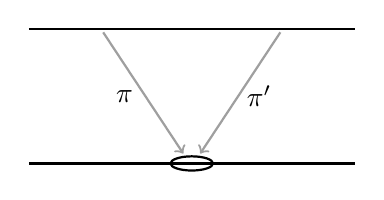
\begin{tikzpicture}[scale=0.9,line width=0.8pt]
  \draw (0,1.9) -- (4.6,1.9);
  \draw (0,0) -- (4.6,0);
  \draw[gray!75,->] (1.05,1.85) -- (2.18,0.14);
  \draw[gray!75,->] (3.55,1.85) -- (2.42,0.14);
  \node at (1.35,0.95) {$\pi$};
  \node at (3.25,0.95) {$\pi'$};
  \draw (2.3,0) ellipse (0.3 and 0.1);
\end{tikzpicture}
\caption{到一个非\trSeparated{}\trScheme{}的两个不同映射在一个稠密开集上相等（见练习 11.3.D）。依原书手绘图重绘。}\label{fig:nonseparated-agreement}
\end{figure}

\textbf{11.3.4.}\ \emph{有理映射的图像。}\quad（\emph{\trMorphism}的图像已在 \S11.2.5 中定义。）若 $X$ 既约而 $Y$ \trSeparated{}，则如下定义\trRationalMap{} $\pi\colon X\dashrightarrow Y$ 的\textbf{图像 $\Gamma_\pi$}（graph）。任取这个\trRationalMap{}的一个代表 $(\mathsf{U},\pi')$（于是 $\pi'\colon\mathsf{U}\to Y$ 是一个\trMorphism）。令 $\Gamma_\pi$ 为 $\Gamma_{\pi'}\hookrightarrow\mathsf{U}\times Y\hookrightarrow X\times Y$ 的\trSchemeTheoretic{}闭包，其中第一个映射是\trClosedEmbedding（命题~11.2.6），第二个映射是\trOpenEmbedding。这里的积应当在你所工作的\trCategory{}中取。例如，如果你处理的是 $k$-\trScheme，纤维积就应当取在 $k$ 上。

\textbf{11.3.E.（练习）}\quad 证明：\trRationalMap{} $\pi\colon X\dashrightarrow Y$ 的图像不依赖于 $\pi$ 之代表的选取。提示：设 $\xi'\colon\mathsf{U}\to Y$ 与 $\xi\colon\mathsf{V}\to Y$ 是 $\pi$ 的两个代表。化归到 $\mathsf{V}$ 是 $\pi$ 的\trDomainOfDefinition（\S11.3.3）且 $\xi'=\xi|_{\mathsf{U}}$ 的情形。再化归到 $\mathsf{V}=X$ 的情形。证明同构 $\Gamma_\pi\cong X$ 与 $\Gamma_{\xi|_{\mathsf{U}}}\cong\mathsf{U}$。（评注：$Y$ 的分离性并不必要。）

类比\trMorphism{}的图像，下面这幅展示\trRationalMap{} $\pi$ 之图像的图示可能会有用（参看\cref{fig:graph-morphism}）。
\[
\begin{tikzcd}[row sep=3em, column sep=3.4em]
\Gamma_\pi \ar[hook, r, "\text{闭嵌入}"] & X\times Y \ar[dr, "\mathrm{pr}_2"] \ar[dl, "\mathrm{pr}_1"] \\
X \ar[u, dotted, "\Upsilon_\pi"'] \ar[rr, dashed, "\pi"] & & Y.
\end{tikzcd}
\]

\textbf{11.3.F.（练习：作为\trRationalMap{}之图像的仿射平面胀开）}\quad 考虑由 $(x,y)\mapsto[x,y]$ 给出的\trRationalMap{} $\mathbb{A}^2_k\dashrightarrow\mathbb{P}^1_k$。证明：这个\trRationalMap{}不能越过原点延拓。（\mbox{练习~7.5.J}中关于\trCremona{}变换的论证与此相类。）证明：这个\trRationalMap{}的图像正是\mbox{练习~10.3.F}所描述的那个\trMorphism（胀开）。（等我们在一般情形下定义胀开时，将会看到它们往往就是\trRationalMap{}的图像；见\mbox{练习~22.4.M}。）

\textbf{11.3.5.\ 变奏。}\quad 定理~11.3.2 那个短证明的种种变奏，可以给出其他有用的结果。\mbox{练习~11.3.B}便是一例。这里是另一例。

\textbf{11.3.G.（练习：到分离概形的映射越过\trEffectiveCartierDivisor{}至多只能以一种方式延拓）}\quad 设 $X$ 是一个 $Z$-\trScheme（不必\trReduced！），而 $Y$ 是一个\trSeparated{}的 $Z$-\trScheme。再设 $D$ 是 $X$ 上的一个\trEffectiveCartierDivisor。证明：任何一个 $Z$-\trMorphism{} $X\setminus D\to Y$ 至多只能以一种方式延拓为 $Z$-\trMorphism{} $X\to Y$。（提示：化归到 $X=\Spec A$ 而 $D$ 为 $t\in A$ 的\trVanishingScheme{}的情形。再化归到证明 $D(t)$ 在 $X$ 中的\trSchemeTheoreticImage{}是整个 $X$。为此可证 $A\to A_t$ 是单的。）

如 \S7.5.2 所述，只要 $X$ 带有\trAssociatedPoint，便可以定义从 $X$ 到任何 $Y$ 的\trRationalMap{}。「既约到分离」定理~11.3.2 可以推广到这一场合，如下。

\textbf{11.3.H.（练习：「相伴到分离」定理（Associated-to-Separated Theorem））}\quad 证明：从一个\trLocally\trNoetherian{}概形 $\mathsf{U}$ 出发、到一个\trSeparated{}的 $S$-\trScheme{} $Z$ 的两个 $S$-\trMorphism{} $\pi$ 与 $\pi'$，若在一个含有 $\mathsf{U}$ 的全部\trAssociatedPoint{}的开子集上相等，则二者相同。


\section{固有态射}

拓扑空间之间的映射（也就是\trContinuousMap！）称为\textbf{固有的}（proper），若任何\trCompact{}集合的原像都是\trCompact{}的。\trMorphism{}的\trProperness{}是一条与之类似的性质。例如，$\mathbb{C}$ 上的一个\trVariety{}若在\trClassicalTopology{}下\trCompact{}，就会是固有的（参看 [Se3, \S7]）。另一方面，我们将会看到：射影 $A$-\trScheme{}都在 $A$ 上固有——所以这是一条射影概形都满足的良好性质，而且用起来也很顺手。

回想（\S8.3.5）：拓扑空间之间的（\trContinuous）映射 $\pi\colon X\to Y$ 称为\emph{闭}的，若对每个闭子集 $S\subset X$，$\pi(S)$ 也是闭的。概形之间的\trMorphism{}称为闭的，若其底下的\trContinuousMap{}是闭的。我们称概形间的\trMorphism{} $\pi\colon X\to Y$ 是\trUniversallyClosed{}的，若对每个\trMorphism{} $Z\to Y$，诱导的\trMorphism{} $Z\times_Y X\to Z$ 都是闭的。换言之，一个\trMorphism{}是泛闭的，若它在任何\trBaseChange{}之下都保持为闭的。事到如今，你大概会自动期待下面这道练习了。

\textbf{11.4.A.（容易的练习）}\quad 证明：泛闭\trMorphism{}构成的类是 \S8.1 意义下的「合理」类。

为给概形的\trProperness{}的定义提供动机，我们指出：设 $\pi\colon X\to Y$ 是局部紧\trHausdorff{}空间之间的一个\trContinuousMap，且二者的拓扑都具有可数\trBase，那么 $\pi$ 是泛闭的，当且仅当它是固有的（即\trCompact{}子集的原像是\trCompact{}的）。欢迎你把这件事当作一道练习证一证。

\textbf{11.4.1.}\ \emph{\trhDefinition{}。}\quad \trMorphism{} $\pi\colon X\to Y$ 称为\textbf{\trProper}的，若它既是\trSeparated{}的、\trFiniteType{}的，又是\trUniversallyClosed{}的。一个\trScheme{} $X$ 常被说成是固有的，若它某个隐含的\trStructureMorphism{}是固有的。例如，一个 $k$-\trScheme{} $X$ 常被描述为固有的，若 $X\to\Spec k$ 是固有的。（固有的 $k$-\trScheme{}也常说成是\textbf{\trComplete}的（complete）。我们不会使用这一术语。）若 $A$ 是一个\trRing，人们常说一个 $A$-\trScheme{}是\textbf{在 $A$ 上固有}的，若它在 $\Spec A$ 上固有。

让我们在实践中把这条观念试用一下。我们预期 $\mathbb{A}^1_{\mathbb{C}}\to\Spec\mathbb{C}$ 不是固有的，因为与 $\mathbb{A}^1_{\mathbb{C}}$ 相应的\trComplex\trManifold{}不是\trCompact{}的。然而请注意：这个映射是\trSeparated{}的（它是仿射概形之间的映射）、\trFiniteType{}的，而且是（平凡地）闭的。所以，关键全在「泛」字上。

\textbf{11.4.B.（容易的练习）}\quad 证明：$\pi\colon\mathbb{A}^1_{\mathbb{C}}\to\Spec\mathbb{C}$ 是一个\trClosed{}映射，但不是泛闭的。从而 $\pi$ 不是固有的。可能的提示：考虑一个精心挑选的映射，比如 $\mathbb{A}^1_{\mathbb{C}}\times_{\mathbb{C}}\mathbb{P}^1_{\mathbb{C}}\to\mathbb{P}^1_{\mathbb{C}}$。（\mbox{图~19.1}给出了另一个有限型、分离、闭、却不固有的\trMorphism{}的例子。而要证明\emph{那个}\trMorphism{}不固有，则需要更多的创造力。）

\textbf{11.4.2.}\ \emph{\trhExample{}。}\quad 作为第一个例子：闭嵌入都是固有的。它们显然\trSeparated，因为仿射\trMorphism{}是\trSeparated{}的（命题~11.2.4）。它们是\trFiniteType{}的。经过\trBaseChange{}之后，它们仍是闭嵌入（\S10.2.2），而闭嵌入总是闭的。这条可以轻易地进一步推广，如下。

\textbf{11.4.3.\ \trhProposition{}。}\ ——\ \emph{有限\trMorphism{}都是固有的。}

\emph{证明。}\ 有限\trMorphism{}是\trSeparated{}的（它们按定义是仿射的，而仿射\trMorphism{}是\trSeparated{}的，命题~11.2.4），并且是\trFiniteType{}的（基本原因：环上的有限\trModule{}自动有限生成）。为证有限\trMorphism{}在任意\trBaseChange{}之后都是闭的，我们注意：它们在任意\trBaseChange{}之后仍是有限的（有限性对\trBaseChange{}保持，\mbox{练习~10.4.D(d)}），而有限\trMorphism{}是闭的（\mbox{练习~8.3.L}）。\hfill$\square$

\textbf{11.4.4.\ \trhProposition{}。}\ ——\ \emph{(a) 「固有\trMorphism」这一观念对\trBaseChange{}稳定。}\\
\emph{(b) 「固有\trMorphism」这一观念是对目标局部的（也就是说，$\pi\colon X\to Y$ 是固有的，当且仅当对任意仿射开覆盖 $\mathsf{U}_i\to Y$，$\pi^{-1}(\mathsf{U}_i)\to\mathsf{U}_i$ 都是固有的）。注意「仅当」方向由 (a) 推出——考虑经 $\mathsf{U}_i\to Y$ 的\trBaseChange{}即可。}\\
\emph{(c) 「固有\trMorphism」这一观念对\trComposition{}保持。}\\
\emph{(d) 两个固有\trMorphism{}的积是固有的：若 $\pi\colon X\to Y$ 与 $\pi'\colon X'\to Y'$ 都是固有的（其中诸\trMorphism{}均为某 $Z$-\trScheme{}之间的\trMorphism），则 $\pi\times\pi'\colon X\times_Z X'\to Y\times_Z Y'$ 是固有的。}\\
\emph{(e) 设}
\begin{equation*}\tag{11.4.4.1}\label{eq:properness-cancellation-triangle}
\begin{tikzcd}[row sep=2.4em, column sep=3.2em]
X \ar[rr, "\pi"] \ar[dr, "\tau"'] & & Y \ar[dl, "\rho"] \\
& Z &
\end{tikzcd}
\end{equation*}
\emph{是一个\trCommutativeDiagram，其中 $\tau$ 是固有的，而 $\rho$ 是\trSeparated{}的。那么 $\pi$ 是固有的。}

(e) 的一个示范应用：从固有的 $k$-\trScheme{}出发、（在 $\Spec k$ 上）到\trSeparated{}的 $k$-\trScheme{}的\trMorphism{}总是固有的。

\emph{证明。}\ (a) 至 (c) 说的是：固有\trMorphism{}构成 \S8.1 意义下的一个「合理」的\trMorphism{}类。于是它们得以成立，因为\trSeparated{}态射、有限型态射与泛闭态射都是「合理」的类。然后，(d) 由 (a) 与 (c) 借\cref{ex:property-product-preserved}推出。闭嵌入是固有的（例~11.4.2），故 (e) 由（对固有\trMorphism{}的）\trCancellationTheorem~11.1.1 推出。\hfill$\square$

\textbf{11.4.C.（练习：「固有概形的像是固有的」）}\quad 设在图
\[
\begin{tikzcd}[row sep=2.4em, column sep=3.2em]
X \ar[rr, "\pi"] \ar[dr, "\tau"'] & & Y \ar[dl, "\rho"] \\
& Z &
\end{tikzcd}
\]
中 $\tau$ 是固有的，而 $\rho$ 是\trSeparated{}且有限型的。证明：$X$ 在 $\pi$ 之下的\trSchemeTheoreticImage{}是一个固有的 $Z$-\trScheme。（由此可见，代数几何中的固有性表现得恰如拓扑中的固有性一样。）

现在我们来看固有态射最重要的例子。

\textbf{11.4.5.\ \trhTheorem{}。}\ ——\ \emph{射影 $A$-\trScheme{}都在 $A$ 上固有。}

（由于到 $\Spec A$ 的有限\trMorphism{}都是射影 $A$-\trScheme{}（\mbox{练习~8.3.I}），定理~11.4.5 可以用来给出「有限\trMorphism{}都是固有的」（命题~11.4.3）的第二个证明。）

\emph{证明。}\ 射影 $A$-\trScheme{}的\trStructureMorphism{} $X\to\Spec A$ 可以分解为一个\trClosedEmbedding{}复合上 $\mathbb{P}^n_A\to\Spec A$。闭嵌入是固有的（例~11.4.2），而固有\trMorphism{}的\trComposition{}是固有的（命题~11.4.4），故只须证明 $\mathbb{P}^n_A\to\Spec A$ 是固有的。我们已经见过这个态射是\trFiniteType{}的（容易练习~5.3.D）且是\trSeparated{}的（命题~11.2.8），故只须证明 $\mathbb{P}^n_A\to\Spec A$ 是泛闭的。由于 $\mathbb{P}^n_A=\mathbb{P}^n_{\mathbb{Z}}\times_{\mathbb{Z}}\Spec A$，只须证明：对任何概形 $X$，$\mathbb{P}^n_X:=\mathbb{P}^n_{\mathbb{Z}}\times_{\mathbb{Z}}X\to X$ 都是闭的。但「闭」这条性质是对目标（此处即 $X$）局部，所以用仿射开子集盖住 $X$ 之后，便只须证明：对一切的环 $B$，$\mathbb{P}^n_B\to\Spec B$ 都是闭的。这正是\trFundamentalTheoremOfEliminationTheory（定理~8.4.10）。\hfill$\square$

\textbf{11.4.6.}\ \emph{\trhRemark{}：}\textbf{「合理」的固有概形都是射影的。}\quad 要举出一个固有却不射影的 $A$-\trScheme{}的例子，可不是件容易事！在域上，所有固有\trCurve{}都是射影的（见注记~19.2.I），所有光滑\trSurface{}都是射影的（\trZariski{}这条定理的证明见 [Ba, Thm.~1.28]；光滑性当然还没定义）。我们将在 \S15.2.11 遇到一个固有却不射影的\trVariety{}（一个奇异三维簇）的第一例。我们日后将在 \S19.11.11 见到一个固有非射影\trSurface{}的例子，并在\mbox{练习~20.2.G}见到一个更简单的。等我们了解了平坦性之后，还将看到\trHironaka{}那个 $\mathbb{C}$ 上固有、非射影、不可约且光滑的三维簇的例子（\S24.7.6）。

\textbf{11.4.7. 连通既约的固有 $\overline{k}$-\trScheme{}上的函数必为常数。}\quad
作为这些观念的一个颇具启发性的应用，我们来证明：若 $X$ 是一个连通、既约、固有的 $k$-\trScheme{}，其中 $k=\overline{k}$，则 $\Gamma(X,\OO_X)=k$。连通\trCompact{}\trComplex\trManifold{}的类似事实用到的是最大值原理（maximum principle）。我们在 $X=\mathbb{P}^n$ 的特殊情形见过它（\mbox{练习~4.4.E}）；它日后将被\trGrothendieck{}凝聚定理~18.9.1（Coherence Theorem）大大地推广。

设 $f\in\Gamma(X,\OO_X)$（$f$ 是 $X$ 上的一个函数）。这与一个映射 $\pi\colon X\to\mathbb{A}^1_k$ 是同一回事（\mbox{练习~7.3.G}，进一步的讨论见 \S7.6.1）。令 $\pi'$ 为 $\pi$ 复合上开嵌入 $\mathbb{A}^1\hookrightarrow\mathbb{P}^1$ 的结果。由命题~11.4.4(e)，$\pi'$ 是固有的，从而特别地是闭的。由于 $X$ 连通，$\pi'$ 的像也连通。于是 $\pi'$ 的集合论像要么是一个闭点，要么是整个 $\mathbb{P}^1$。但 $\pi'$ 的集合论像落在 $\mathbb{A}^1$ 中，故它必是一个闭点 $p$（我们把它与 $k$ 的一个元素相认同）。

由推论~9.4.5，$\pi$ 的\trSchemeTheoreticImage{}的\trSupport{}是这个闭点 $p$。由\mbox{练习~9.4.A}，\trSchemeTheoreticImage{}恰好就是 $p$（带既约结构）。于是 $\pi$ 可以解读为：先取到 $\Spec k$ 的\trStructureMorphism，再复合一个把 $\Spec k$ 认同于 $p$ 的、到 $\mathbb{A}^1$ 的闭嵌入。你应当能够验证：这正是对应于常值函数 $f=p$ 的那个到 $\mathbb{A}^1$ 的映射。

（若放松不同的假设，反例为何？条件 $k=\overline{k}$ 是不可忽视的——若 $k=\mathbb{R}$，则 $X=\Spec\mathbb{C}$ 是一个连通既约的固有射影 $k$-\trScheme，而 $\Gamma(X,\OO_X)=k^2$。一个有趣的事实：$\mathbb{P}^2_k$ 中 $x^2=0$ 表明，即便是非既约的固有 $k$-\trScheme，其上的函数也可以只有常数；见 \S5.2.3 与\mbox{练习~18.6.U}。）

\textbf{11.4.8. 或许能帮助你正确思考有限性的若干事实（尚未证明）。}\quad
下面的几条事实或许能照亮「有限性」这个观念。我们日后再证明它们。

\trLocally\trNoetherian{}概形之间的\trMorphism{}是有限的，当且仅当它既固有又仿射，当且仅当它既固有又拟有限（定理~28.5.2）。这个陈述的若干部分我们已经证过，但只有等到我们知道\trZariskiMainTheorem{}之后，才能完成整个证明；对比 \S8.3.12。

作为一个应用：从固有概形到分离概形的拟有限\trMorphism{}是有限的。道理如下：设 $\pi\colon X\to Y$ 是 $Z$ 上的一个拟有限\trMorphism，其中 $X$ 在 $Z$ 上固有。那么由（对固有\trMorphism{}的）\trCancellationTheorem~11.1.1，$X\to Y$ 是固有的。于是既然 $\pi$ 既拟有限又固有，$\pi$ 就是有限的。

作为一个显式的例子，考虑由 $[x,y]\mapsto[f(x,y),\,g(x,y)]$ 给出的映射 $\pi\colon\mathbb{P}^1_k\to\mathbb{P}^1_k$，其中 $f$ 与 $g$ 是次数相同、且在 $\mathbb{P}^1$ 中没有公共根的齐次多项式。诸\trFiber{}有限，而 $\pi$ 是固有的（由对固有\trMorphism{}的\trCancellationTheorem~11.1.1，如命题~11.4.4\footnote{原书此处作（Theorem 11.4.4），而 11.4.4 实为命题，当系「命题」之误，径改。——译者注} 之后所讨论的那样），故 $\pi$ 是有限的。这件事固然也可以直接验证，但现在我们可以省去这份烦冗了。

\textbf{11.4.9.}\ \extrahard\ \textbf{\trGroupVariety{}。}\quad \S11.4 的其余部分都是双星的，而且我们也将通盘在域 $k$ 上的\emph{\trVariety}这一\trCategory{}中工作。我们简短地讨论\trGroupVariety{}，主要是因为力所能及，而不是因为我们有什么深刻的见地要说。之所以此刻就把它们拿出来讨论，只是因为固有性给出一条出人意料的推论：固有的\trGroupVariety{}是\trAbelian{}的（多亏出奇简单的刚性引理~11.4.12）。

如 \S11.2.9 所讨论的，既然我们手里已有域 $k$ 上的簇这一\trCategory{}，便立即有了\textbf{\trGroupVariety{}}（group variety）的观念（多谢 \S7.6.4 讲的任意\trCategory{}中的\trGroupObject）。一个（$k$ 上的）\textbf{\trAlgebraic\trGroup}（algebraic group）是一个光滑的\trGroupVariety{}。例子包括 $\mathrm{GL}_n$（\mbox{练习~7.6.N(b)}）——$\mathbb{G}_m$ 是其特例——以及 $\mathrm{SL}_n$（\mbox{练习~7.6.Q}）。

\textbf{11.4.10.}\ \emph{旁注}（我们既不证明也不使用）。\quad \trGroupVariety{}在特征 $0$ 时自动光滑（从而是\trAlgebraicGroup{}）。\trGroupVariety{}在正特征下未必光滑。（设 $k$ 是特征 $p$ 的不\trPerfectField，取 $t\in k$ 使其在 $k$ 中没有 $p$ 次根。考虑「加法群」（additive group）$\mathbb{G}_a^2=\Spec k[x,y]$ 中由 $x^p=ty^p$ 给出的「闭子群概形」。这个群概形既约，却不几何既约；而且不光滑，甚至连正则都不是。）\trAlgebraicGroup{}自动拟射影。\trAlgebraicGroup{} $G$ 是仿射的（作为概形），当且仅当它能容纳一个到某 $\mathrm{GL}_n$（$n\ge 0$）的\trClosedImmersion{}，使得 $G\to\mathrm{GL}_n$ 是群概形之间的同态（\mbox{练习~7.6.N(a)}）。关于这些问题与其他议题的进一步讨论，见 [P2, \S5]。

\textbf{11.4.11.}\ \emph{\trhDefinition{}：}\textbf{\trAbelianVariety{}}。\quad 我们现在可以定义\trVariety{}最重要的类之一了：\trAbelianVariety{}（abelian variety）。坏消息是，我们还没有一个真正的例子。我们日后将见到椭圆曲线作为一例（\S19.10），但比它更奇特的例子我们就无缘得见了。尽管如此，能这么早就作出这个定义，还是令人愉快的。

域 $k$ 上的一个\textbf{\trAbelian\trVariety}（abelian variety）是一个几何整且（在 $k$ 上）射影的\trAlgebraicGroup{}。事实证明，$\mathbb{C}$ 上任何\trAbelianVariety{}的\trAnalytification{}都是一个\trComplexTorus{}（complex torus），也就是说形如 $\mathbb{C}^n/\Lambda$，其中 $\Lambda$ 是一个\trLattice{}（lattice）（秩为 $2n$）。（关键想法：连通\trCompact{}\trComplex{}\trLie{}群是交换的；见注记~11.4.14；其\trUniversalCover{}（universal cover）是一个\trSimplyConnected{}（simply connected）的交换复\trLie{}群，从而是 $\mathbb{C}^n$。参看 [BL, Lem.~1.1.1]。）

我们现在来证明：\trAbelianVariety{}是\trAbelian{}的，也就是说，\trAbelianVariety{}是交换的代数\trGroupVariety{}。（这话听起来像同义反复，其实不然！形容词「阿贝尔」用于两种不同的意义；二者的共同点是：它们都源自 Niels Henrik Abel（尼尔斯·亨利克·阿贝尔）之名。）由于\trAlgebraicGroup{}未必交换（$\mathrm{GL}_n$ 便是见证），交换性竟能被「紧致性」逼出来，这就多少令人称奇了。

关键的结果是下面这个事实，它本身就美得很。

\textbf{11.4.12.\ 刚性引理}（Rigidity Lemma）\textbf{。}\ ——\ \emph{设 $X$、$Y$、$Z$ 都是\trVariety，其中 $X$ 固有且\trGeometricallyIntegral，并带有一个 $k$-\trValuedPoint{} $p$，而 $Y$ 不可约。设 $\mathrm{pr}\colon X\times Y\to Y$ 是\trProjection，而 $\alpha\colon X\times Y\to Z$ 是任一\trMorphism。设 $q\in Y$ 使得 $\alpha$ 在 $X\times\{q\}$ 上为常值；比如说 $\alpha(X\times\{q\})=r\in Z$。}\\
\emph{(a) 那么存在\trMorphism{} $\psi\colon Y\to Z$ 使 $\alpha=\psi\circ\mathrm{pr}$。（特别地，对每个 $q'\in Y$，$\alpha$ 在 $X\times\{q'\}$ 上为常值。）}\\
\emph{(b) 若 $\alpha$ 在 $\{p\}\times Y$ 上也为常值，则 $\alpha$ 在整个 $X\times Y$ 上都是常值的。}

\[
\begin{tikzcd}[row sep=3em, column sep=3.6em]
& & Z \\
X\times\{q\} \ar[r] \ar[d] & X\times Y \ar[ur, "\alpha"] \ar[d, "\mathrm{pr}"', shift left=0.55em] \\
q \ar[r] & Y \ar[u, "\sigma_p"', shift right=0.55em] \ar[uur, bend right=24, "\psi"]
\end{tikzcd}
\]

这些假设可以在许多方向上放松，但这个版本对我们的目的已经够用。如果你没有读过讨论几何整性的 \S10.5.1，也不必过于担心；当 $k=\overline{k}$ 且 $X$ 是整的时候，它是自动成立的（「更难事实」~10.5.3）。即便你读过 \S10.5.1，先在 $k=\overline{k}$ 的假定下读这个证明也会很有帮助，以免被几何点岔开对主要想法的注意力。但话又说回来，\S11.4.9 的全部内容都是双星的，所以你本来就不该读到这里的。

\textbf{11.4.D.（练习）}\quad 证明：$X$ 的固有性假设是必要的。（你能让这与你的直觉相安无事吗？）

\emph{刚性引理~11.4.12 的证明。}\ 定义 $\beta\colon X\times Y\to Z$ 为 $\beta(x,y)=\alpha(p,y)$。（更精确地说，若 $\sigma_p$ 是从 $\Spec k\hookrightarrow p$ 拉回的 $X\times Y\to Y$ 的\trSection，则 $\beta=\alpha\circ\sigma_p\circ\mathrm{pr}$。）我们将证明 $\beta(x,y)=\alpha(x,y)$。这将蕴涵 (a)（取 $\psi=\alpha\circ\sigma_p$），而 (a) 又立即蕴涵 (b)。

命题~10.5.19（几何既约乘既约是既约）蕴涵 $X\times Y$ 是既约的。\mbox{练习~10.5.O}（几何不可约乘不可约是不可约）蕴涵 $X\times Y$ 是不可约的。由于 $Z$ 是分离的，由\mbox{练习~11.3.A}，只须证明 $\alpha=\beta$ 在 $X\times Y$ 的某个非空（从而稠密）开子集上成立。

设 $\mathsf{U}\subset Z$ 是 $r$ 的一个仿射开邻域。那么 $\alpha^{-1}(Z\setminus\mathsf{U})$ 是 $X\times Y$ 的闭子集。由于\trProjection $\mathrm{pr}$ 是固有的（利用 $X$ 的固有性，以及固有性在\trBaseChange{}下的保持，命题~11.4.4(a)），$\mathrm{pr}(\alpha^{-1}(Z\setminus\mathsf{U}))$ 是闭的。它的补集是开的，并且含有 $q$；令 $\mathsf{V}\subset Y$ 是 $q$ 的一个开邻域，与 $\mathrm{pr}(\alpha^{-1}(Z\setminus\mathsf{U}))$ 不相交。

\textbf{11.4.E.（练习）}\quad 设 $\gamma\colon\Spec\overline{K}\to\mathsf{V}$ 是 $\mathsf{V}$ 的一个\trGeometricPoint。证明：$\Spec\overline{K}$ 之上的纤维 $X_{\overline{K}}$（或者更精确地说，$\gamma$ 之上的纤维）被 $\alpha$ 限制在 $X_{\overline{K}}$ 上的 $\alpha_{\overline{K}}$ 送到 $Z$ 中的一个点。提示：重温 \S11.4.7。
\[
\begin{tikzcd}[row sep=3em, column sep=3.8em]
& & Z \\
X_{\overline{K}} \ar[rr] \ar[d] \ar[urr, "\alpha_{\overline{K}}", shift left=0.5em] & & X\times\mathsf{V} \ar[u, "\beta_{\overline{K}}", shift left=0.5em] \ar[u, bend right=30, "\alpha|_{\mathsf{V}}"'] \ar[d, "\mathrm{pr}"'] \\
\Spec\overline{K} \ar[rr, "\gamma"'] & & \mathsf{V}
\end{tikzcd}
\]
由\mbox{练习~11.3.B}（代数闭域上的簇由闭点上的映射决定），$\alpha_{\overline{K}}=\beta_{\overline{K}}$。

\textbf{11.4.F.（练习）}\quad 用\mbox{练习~11.3.A}（$\alpha=\beta$ 之处是一个\trClosedSubscheme{}这一事实——而且它表示某个函子）证明：在 $\mathrm{pr}^{-1}(\mathsf{V})$ 上有 $\alpha=\beta$。\hfill$\square$

\textbf{11.4.13.\ \trhCorollary{}。}\ ——\ \emph{设 $A$ 是一个\trAbelian\trVariety，$G$ 是一个\trGroup\trVariety，而 $\phi\colon A\to G$ 是\trVariety{}之间的任一\trMorphism。那么 $\phi$ 是一个\trTranslation{}（translation）与一个同态的复合。}

\emph{证明。}\ 设 $\mathrm{e}_A$ 与 $\mathrm{e}_G$ 分别是 $A$ 与 $G$ 的\trIdentityPoint{}（identity point）。把 $\phi$ 复合上一个\trTranslation{}，便可设 $\phi(\mathrm{e}_A)=\mathrm{e}_G$。考虑由 $\alpha(a_1,a_2)=\phi(a_1a_2)\phi(a_2)^{-1}\phi(a_1)^{-1}$ 给出的\trMorphism{} $\alpha\colon A\times A\to G$。那么 $\alpha(\{\mathrm{e}_A\}\times A)=\alpha(A\times\{\mathrm{e}_A\})=\{\mathrm{e}_G\}$，故由刚性引理~11.4.12，$\alpha$ 是常值的，并把 $A\times A$ 送到 $\mathrm{e}_G$。于是 $\phi(a_1a_2)=\phi(a_1)\phi(a_2)$，故 $\phi$ 是一个同态。\hfill$\square$

\textbf{11.4.G.（练习：\trAbelianVariety{}是\trAbelian{}的）}\quad 证明：\trAbelianVariety{}是一个\trAbelian{}的\trGroupVariety{}。提示：把推论~11.4.13 应用到求逆\trMorphism{} $i\colon A\to A$ 上。

\textbf{11.4.14.}\ \emph{\trhRemark{}。}\quad 类似的想法还被用来证明：连通\trCompact{}\trComplex{}\trLie{}群是\trAbelian{}的；例如参看 [BL, Lem.~1.1.1]。

